% The two harness stacks, stage by stage, colored by state. Redraw as the build moves:
% the state of each chip is the first argument of \chip (main, copy, wip).
% Build: pdflatex stack-map.tex
\documentclass[border=8pt]{standalone}
\usepackage[T1]{fontenc}
\usepackage[default]{sourcesanspro}
\usepackage[scaled=0.92]{inconsolata}
\usepackage{tikz}
\definecolor{wrap}{HTML}{92C7E7}
\definecolor{light}{HTML}{D6EAF6}
\definecolor{edge}{HTML}{2F5B7C}
\definecolor{navy}{HTML}{14273A}
\definecolor{mid}{HTML}{5B6670}
% \chip{state}{x}{y}{name}{code}{loop dot: 1 or 0}
\newcommand{\chip}[6]{%
  \path[#1] (#2,#3)--++(2.5,0)--++(0,0.84)--++(-0.26,0.26)--++(-1.98,0)--++(-0.26,-0.26)--cycle;
  \node[font=\bfseries\small,text=navy,anchor=south] at ({#2+1.25},{#3+0.5}) {#4};
  \node[font=\ttfamily\scriptsize,text=mid,anchor=north] at ({#2+1.25},{#3+0.54}) {#5};
  \ifnum#6=1 \fill[navy] ({#2+2.27},{#3+0.93}) circle (0.075); \fi}
\begin{document}
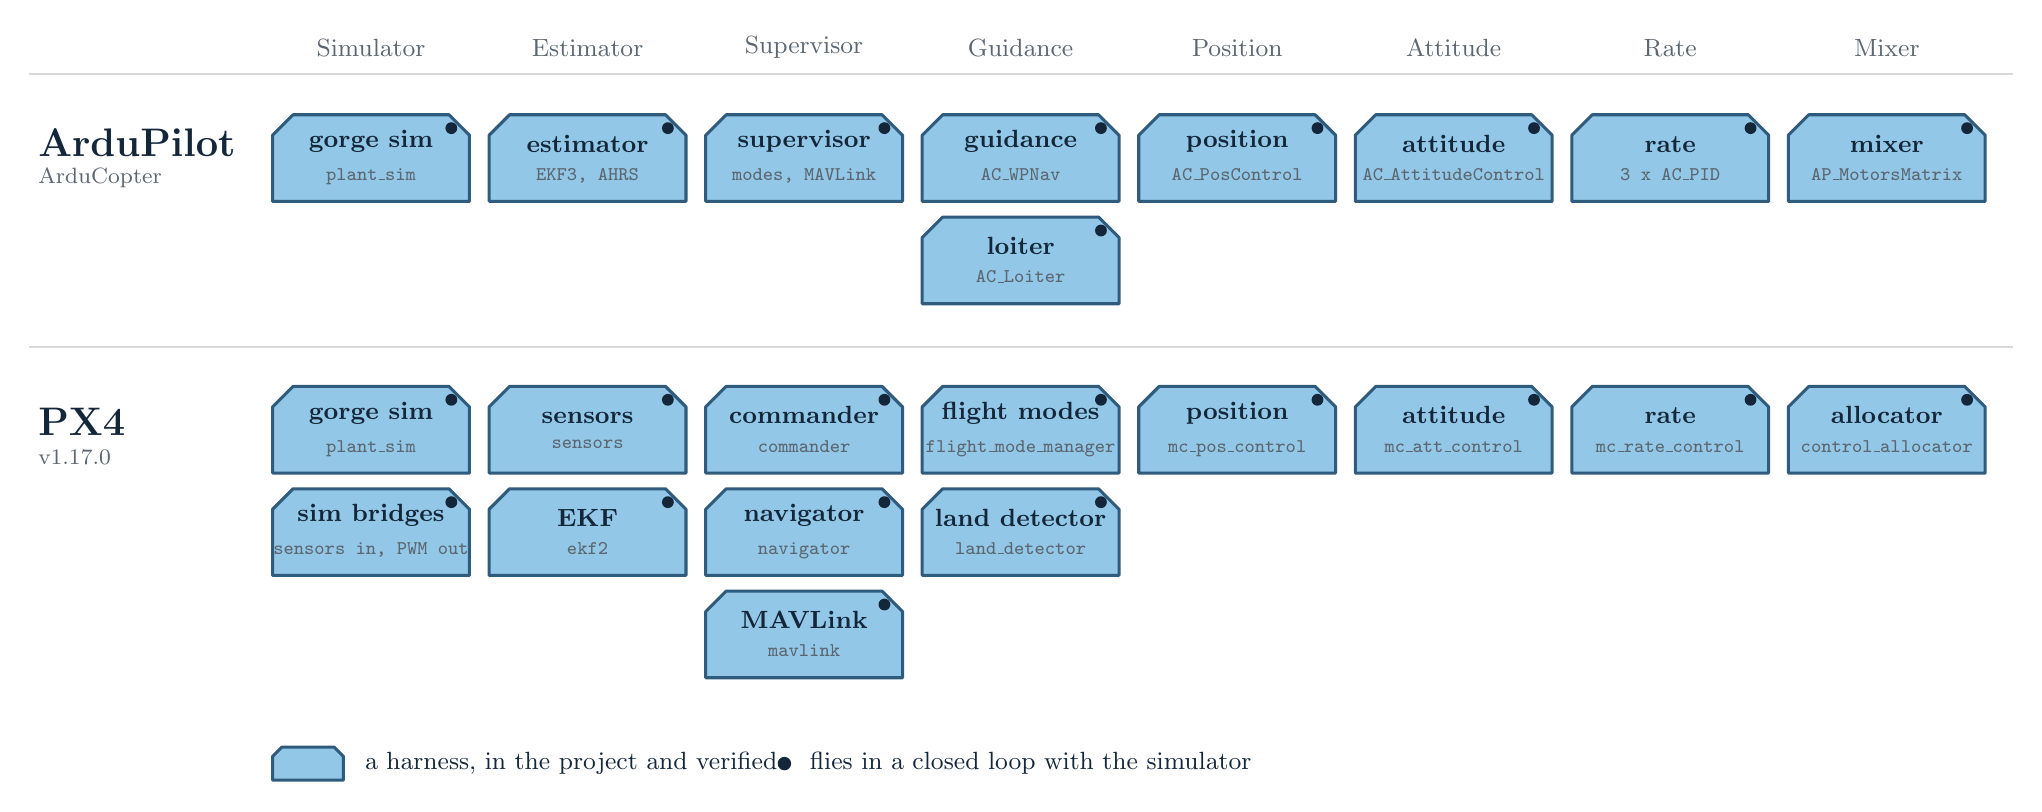
\begin{tikzpicture}[x=1cm,y=1cm,line join=round,
  main/.style={fill=wrap,draw=edge,line width=1.1pt},
  copy/.style={fill=light,draw=edge,line width=1.1pt},
  wip/.style={fill=white,draw=edge,line width=0.9pt,dash pattern=on 3pt off 2pt}]
% column headers
\foreach \i/\h in {0/Simulator,1/Estimator,2/Supervisor,3/Guidance,4/Position,5/Attitude,6/Rate,7/Mixer}{
  \node[font=\small,text=mid] at ({3.1+\i*2.75+1.25},8.05) {\h};}
\draw[black!15,line width=0.6pt] (0,7.72)--(25.2,7.72);
\draw[black!15,line width=0.6pt] (0,4.25)--(25.2,4.25);

% ---------------- ArduPilot
\node[font=\bfseries\Large,text=navy,anchor=west] at (0,6.85) {ArduPilot};
\node[font=\footnotesize,text=mid,anchor=west] at (0,6.4) {ArduCopter};
\chip{main}{3.1}{6.1}{gorge sim}{plant\_sim}{1}
\chip{main}{5.85}{6.1}{estimator}{EKF3, AHRS}{1}
\chip{main}{8.6}{6.1}{supervisor}{modes, MAVLink}{1}
\chip{main}{11.35}{6.1}{guidance}{AC\_WPNav}{1}
\chip{main}{11.35}{4.8}{loiter}{AC\_Loiter}{1}
\chip{main}{14.1}{6.1}{position}{AC\_PosControl}{1}
\chip{main}{16.85}{6.1}{attitude}{AC\_AttitudeControl}{1}
\chip{main}{19.6}{6.1}{rate}{3 x AC\_PID}{1}
\chip{main}{22.35}{6.1}{mixer}{AP\_MotorsMatrix}{1}

% ---------------- PX4
\node[font=\bfseries\Large,text=navy,anchor=west] at (0,3.3) {PX4};
\node[font=\footnotesize,text=mid,anchor=west] at (0,2.85) {v1.17.0};
\chip{main}{3.1}{2.65}{gorge sim}{plant\_sim}{1}
\chip{main}{3.1}{1.35}{sim bridges}{sensors in, PWM out}{1}
\chip{main}{5.85}{2.65}{sensors}{sensors}{1}
\chip{main}{5.85}{1.35}{EKF}{ekf2}{1}
\chip{main}{8.6}{2.65}{commander}{commander}{1}
\chip{main}{8.6}{1.35}{navigator}{navigator}{1}
\chip{main}{8.6}{0.05}{MAVLink}{mavlink}{1}
\chip{main}{11.35}{2.65}{flight modes}{flight\_mode\_manager}{1}
\chip{main}{11.35}{1.35}{land detector}{land\_detector}{1}
\chip{main}{14.1}{2.65}{position}{mc\_pos\_control}{1}
\chip{main}{16.85}{2.65}{attitude}{mc\_att\_control}{1}
\chip{main}{19.6}{2.65}{rate}{mc\_rate\_control}{1}
\chip{main}{22.35}{2.65}{allocator}{control\_allocator}{1}

% ---------------- legend
\path[main] (3.1,-1.25)--++(0.9,0)--++(0,0.3)--++(-0.12,0.12)--++(-0.66,0)--++(-0.12,-0.12)--cycle;
\node[anchor=west,font=\small,text=navy] at (4.15,-1.04) {a harness, in the project and verified};
\fill[navy] (9.6,-1.04) circle (0.085);
\node[anchor=west,font=\small,text=navy] at (9.8,-1.04) {flies in a closed loop with the simulator};
\end{tikzpicture}
\end{document}
